\chapter{Insiemi finiti e calcolo combinatorio}\label{cap:finiti}

Con i numeri naturali possiamo finalmente \textbf{contare}: definire quanti elementi ha un insieme finito e calcolare quante
sono le funzioni, le funzioni iniettive, le biezioni tra due insiemi finiti e le parti di un insieme. Vedremo anche che negli
insiemi finiti iniettività, suriettività e biettività coincidono (per funzioni tra insiemi con lo stesso numero di elementi), e
ne ricaveremo due fatti sulle strutture algebriche finite lasciati in sospeso nella Parte~III.

% ──────────────────────────────────────────────────────────────
\section{Insiemi finiti}\label{sec:finiti}

\dfn[finito]{Segmenti iniziali, insieme finito, ordine}{
    Poniamo $I_0 := \varnothing$ e, per $n \in \mbN \setminus \{0\}$, $I_n := \{1, 2, \dots, n\} = \{k \in \mbN \mid 1 \leq k \leq n\}$: sono i
    \textbf{segmenti iniziali} di $\mbN \setminus \{0\}$. Un insieme $a$ si dice \textbf{finito} se è equipotente a $I_n$ per qualche
    $n \in \mbN$; $n$ si dice \textbf{ordine} (o \textbf{cardinalità}) di $a$ e si scrive $|a| = n$.
}

Contare gli elementi di $a$ vuol dire proprio costruire una biezione $I_n \to a$: «il primo, il secondo, \dots, l'$n$-esimo».
Ad esempio $|a| = 0$ significa che esiste una biezione $a \to I_0 = \varnothing$, il che obbliga $a = \varnothing$ (se $a$ avesse un
elemento, la funzione non saprebbe dove mandarlo). Perché la definizione di ordine abbia senso, bisogna escludere che uno stesso
insieme sia equipotente a due segmenti diversi: segue dal teorema seguente.

\begin{concetto}
\begin{Teorema}{I segmenti iniziali non sono infiniti}{in-non-infinito}
    \begin{prerequisiti}
        \dip{Definizione}{def:finito}
        \dip{Definizione}{def:infinito}
        \dip{Corollario}{cor:induzione-uso}
        \dip{Definizione}{def:funzioni-notevoli}
    \end{prerequisiti}
    Per ogni $n \in \mbN$, $I_n$ non è infinito: non esiste una biezione tra $I_n$ e una sua parte propria.
\end{Teorema}
\begin{dimostrazione}
    Per induzione su $n$. \textbf{Base}: $I_0 = \varnothing$ non ha parti proprie. \textbf{Passo}: supponiamo che $I_n$ non sia infinito e,
    per assurdo, sia $f \colon I_{n + 1} \to x$ biettiva con $x \subset I_{n + 1}$ parte propria.
    \begin{caso}{Caso 1: $n + 1 \notin x$}
        Allora $x \subseteq I_n$ e la restrizione $f_{|I_n}$ è una biezione tra $I_n$ e $x \setminus \{f(n + 1)\}$, che è una parte propria di $I_n$
        (le manca almeno $f(n + 1) \in I_n$). Assurdo per l'ipotesi induttiva.
    \end{caso}
    \begin{caso}{Caso 2: $n + 1 \in x$ e $f(n + 1) = n + 1$}
        Allora $f_{|I_n}$ è una biezione tra $I_n$ e $x \setminus \{n + 1\}$, che è una parte propria di $I_n$ (perché $x \neq I_{n + 1}$). Assurdo.
    \end{caso}
    \begin{caso}{Caso 3: $n + 1 \in x$ e $f(n + 1) = h \neq n + 1$}
        Sia $k \in I_n$ l'elemento con $f(k) = n + 1$. La funzione $g$ che coincide con $f$ su $I_n \setminus \{k\}$ e manda $k$ in $h$ è una
        biezione tra $I_n$ e $x \setminus \{n + 1\}$, parte propria di $I_n$. Assurdo.
    \end{caso}
\end{dimostrazione}
\end{concetto}

\begin{spiegazione}
    L'idea è ridursi da $I_{n + 1}$ a $I_n$ \textbf{togliendo l'ultimo elemento} da entrambe le parti, in modo da usare l'ipotesi
    induttiva. Se $f$ manda $n + 1$ in sé stesso basta tagliarlo via (caso 2); se lo manda altrove, prima si «aggiusta» $f$
    scambiando due frecce, come in figura per $n + 1 = 4$ (caso 3):
    \begin{center}
    \begin{tikzpicture}
        \foreach \i in {1,...,4} { \node[elem] (a\i) at (0,-\i*0.6) {$\i$}; \node[elem] (b\i) at (2.4,-\i*0.6) {$\i$}; }
        \draw[fun] (a1) -- (b2); \draw[fun] (a2) -- (b4); \draw[fun] (a3) -- (b1); \draw[fun2] (a4) -- (b3);
        \node[font=\small] at (1.2,-3.0) {$f \colon I_4 \to x = I_4$};
        \draw[-{Stealth}, line width=0.9pt, primary] (3.3,-1.5) -- node[above, font=\small] {aggiusto} (4.7,-1.5);
        \begin{scope}[xshift=5.6cm]
            \foreach \i in {1,...,3} { \node[elem] (c\i) at (0,-\i*0.6) {$\i$}; \node[elem] (d\i) at (2.4,-\i*0.6) {$\i$}; }
            \node[elem, black!30] at (0,-2.4) {$4$}; \node[elem, black!30] at (2.4,-2.4) {$4$};
            \draw[fun] (c1) -- (d2); \draw[fun3, line width=1pt] (c2) -- (d3); \draw[fun] (c3) -- (d1);
            \node[font=\small, align=center] at (1.2,-3.15) {$g \colon I_3 \to I_3$: $2$ va in $3 = f(4)$\\ al posto di $4 = f(2)$};
        \end{scope}
    \end{tikzpicture}
    \end{center}
    Il disegno mostra il meccanismo di aggiustamento su una biezione di $I_4$ in sé: $f(4) = 3$ e $f(2) = 4$; la $g$ manda $2$ in $3$ e
    dimentica $4$. Nella dimostrazione lo stesso aggiustamento produrrebbe una biezione di $I_n$ su una sua parte propria, che per
    l'ipotesi induttiva non esiste.
\end{spiegazione}

Ne seguono le proprietà che rendono il contare affidabile. Per dimostrarle servono due lemmi su come cambia l'ordine
togliendo o aggiungendo un elemento.

\begin{concetto}
\begin{Lemma}{Togliere o aggiungere un elemento}{togli-elemento}
    \begin{prerequisiti}
        \dip{Definizione}{def:finito}
        \dip{Corollario}{cor:comp-biettive}
    \end{prerequisiti}
    \begin{enumerate}
        \item Se $|a| = n \geq 1$ e $x \in a$, allora $|a \setminus \{x\}| = n - 1$.
        \item Se $|b| = n$ e $x \notin b$, allora $|b \cup \{x\}| = n + 1$.
    \end{enumerate}
\end{Lemma}
\begin{dimostrazione}
    \begin{caso}{Punto 1}
        Sia $f \colon a \to I_n$ biettiva e sia $\tau \colon I_n \to I_n$ la funzione che scambia $f(x)$ e $n$ e lascia fermi gli altri numeri
        ($\tau \circ \tau = \mathrm{id}$, quindi $\tau$ è biettiva). Allora $g = \tau \circ f$ è biettiva e $g(x) = n$. La restrizione di $g$ ad
        $a \setminus \{x\}$ è iniettiva e prende tutti i valori di $I_n$ tranne $n$: è una biezione tra $a \setminus \{x\}$ e $I_{n - 1}$.
    \end{caso}
    \begin{caso}{Punto 2}
        Se $f \colon b \to I_n$ è biettiva, la funzione che coincide con $f$ su $b$ e manda $x$ in $n + 1$ è una biezione tra $b \cup \{x\}$ e $I_{n + 1}$.
    \end{caso}
\end{dimostrazione}
\end{concetto}

\begin{spiegazione}
    Se abbiamo numerato gli elementi di $a$ da $1$ a $n$ e vogliamo togliere $x$, scambiamo il numero di $x$ con quello
    dell'ultimo elemento e poi togliamo l'ultimo: i numeri rimasti sono ancora $1, \dots, n - 1$, senza buchi. Per aggiungere un
    elemento basta dargli il numero $n + 1$.
\end{spiegazione}

\begin{concetto}
\begin{Lemma}{Le parti di un insieme finito sono finite}{parti-finite}
    \begin{prerequisiti}
        \dip{Lemma}{lem:togli-elemento}
        \dip{Corollario}{cor:induzione-uso}
    \end{prerequisiti}
    Se $s$ è finito e $t \subseteq s$, allora $t$ è finito e $|t| \leq |s|$.
\end{Lemma}
\begin{dimostrazione}
    Per induzione su $n = |s|$. \textbf{Base}: se $|s| = 0$, allora $s = \varnothing$ e $t = \varnothing$. \textbf{Passo}: sia $|s| = n + 1$, sia
    $x \in s$ e $s' = s \setminus \{x\}$, che ha ordine $n$ (Lemma~\ref{lem:togli-elemento}).
    Se $x \notin t$, allora $t \subseteq s'$ e per ipotesi induttiva $|t| \leq n \leq n + 1$. Se $x \in t$, allora $t \setminus \{x\} \subseteq s'$, che
    per ipotesi induttiva ha ordine $k \leq n$, e $|t| = k + 1 \leq n + 1$ per il Lemma~\ref{lem:togli-elemento}, punto 2.
\end{dimostrazione}
\end{concetto}

\begin{spiegazione}
    Si guarda un elemento $x$ alla volta: o resta fuori da $t$, o entra in $t$; in entrambi i casi $t$ «guadagna» al più un
    elemento rispetto a una parte di un insieme più piccolo. Sembra ovvio, ma è proprio questo che ci autorizza a dire che una
    parte ha al più tanti elementi quanti l'insieme.
\end{spiegazione}

\begin{concetto}
\begin{Teorema}{L'ordine di un insieme finito}{ordine-finito}
    \begin{prerequisiti}
        \dip{Teorema}{teo:in-non-infinito}
        \dip{Lemma}{lem:parti-finite}
        \dip{Proposizione}{prop:equipotenza}
    \end{prerequisiti}
    \begin{enumerate}
        \item Se $a$ è equipotente sia a $I_m$ sia a $I_n$, allora $m = n$: l'ordine di un insieme finito è ben definito.
        \item Un insieme finito non è infinito.
        \item Se $t$ è una parte \textbf{propria} di un insieme finito $s$, allora $|t| < |s|$.
    \end{enumerate}
\end{Teorema}
\begin{dimostrazione}
    Il punto 2 il programma lo indica senza dimostrazione; la diamo comunque perché serve per il punto 3.
    \begin{caso}{Punto 1}
        $I_m$ e $I_n$ sono equipotenti (Proposizione~\ref{prop:equipotenza}). Se fosse ad esempio $m < n$, $I_m$ sarebbe una parte propria di
        $I_n$ equipotente a $I_n$, e $I_n$ sarebbe infinito, contro il Teorema~\ref{teo:in-non-infinito}.
    \end{caso}
    \begin{caso}{Punto 2}
        Sia $f \colon s \to I_n$ biettiva e, per assurdo, $g \colon s \to t$ biettiva con $t \subset s$. Allora $f \circ g \circ f^{-1}$ è una biezione tra
        $I_n$ e $\overrightarrow{f}(t)$, che è una parte propria di $I_n$ (se $y \in s \setminus t$, $f(y) \notin \overrightarrow{f}(t)$ perché $f$ è
        iniettiva). Assurdo per il Teorema~\ref{teo:in-non-infinito}.
    \end{caso}
    \begin{caso}{Punto 3}
        Per il Lemma~\ref{lem:parti-finite} $|t| \leq |s|$. Se fosse $|t| = |s| = n$, $s$ e $t$ sarebbero entrambi equipotenti a $I_n$, quindi tra loro:
        $s$ sarebbe equipotente alla sua parte propria $t$, cioè infinito, contro il punto 2.
    \end{caso}
\end{dimostrazione}
\end{concetto}

\begin{spiegazione}
    Questi tre fatti sono il «contratto» del contare: contando gli stessi oggetti in due ordini diversi si ottiene lo stesso numero
    (punto 1), e togliendo qualcosa a un insieme finito il numero scende davvero (punto 3). Con gli insiemi infiniti il punto 3 è
    falso: $\mbN \setminus \{0\}$ è una parte propria di $\mbN$ ma i due sono equipotenti (albergo di Hilbert, Esempio~\ref{es:hilbert}).
\end{spiegazione}

% ──────────────────────────────────────────────────────────────
\section{Unioni e prodotti di insiemi finiti}\label{sec:unioni-finite}

\begin{concetto}
\begin{Lemma}{Unione disgiunta e prodotto cartesiano}{somma-prodotto}
    \begin{prerequisiti}
        \dip{Lemma}{lem:togli-elemento}
        \dip{Corollario}{cor:induzione-uso}
        \dip{Definizione}{def:prodotto-cartesiano}
    \end{prerequisiti}
    Siano $a$ e $b$ insiemi finiti.
    \begin{enumerate}
        \item Se $a \cap b = \varnothing$, allora $|a \cup b| = |a| + |b|$.
        \item $|a \times b| = |a| \cdot |b|$.
        \item Se $p = \{w_1, \dots, w_r\}$ è una partizione di un insieme finito $c$ in $r$ blocchi, allora $|c| = |w_1| + \dots + |w_r|$; in particolare,
              se tutti i blocchi hanno $k$ elementi, $|c| = rk$.
    \end{enumerate}
\end{Lemma}
\begin{dimostrazione}
    \begin{caso}{Punto 1, per induzione su $|b|$}
        Se $|b| = 0$, $a \cup \varnothing = a$. Se $|b| = k + 1$, sia $y \in b$ e $b' = b \setminus \{y\}$: per ipotesi induttiva $|a \cup b'| = |a| + k$;
        inoltre $y \notin a \cup b'$ (perché $a \cap b = \varnothing$), quindi $|a \cup b| = |(a \cup b') \cup \{y\}| = |a| + k + 1$.
    \end{caso}
    \begin{caso}{Punto 2, per induzione su $|b|$}
        Se $b = \varnothing$, $a \times b = \varnothing$. Altrimenti, con $y$ e $b'$ come sopra, $a \times b = (a \times b') \cup (a \times \{y\})$, unione
        disgiunta; $x \mapsto (x, y)$ è una biezione tra $a$ e $a \times \{y\}$, quindi per il punto 1 $|a \times b| = |a| \cdot |b'| + |a| = |a|(|b'| + 1)$.
    \end{caso}
    \begin{caso}{Punto 3, per induzione su $r$}
        I blocchi sono a due a due disgiunti, quindi si aggiunge un blocco alla volta e si applica il punto 1.
    \end{caso}
\end{dimostrazione}
\end{concetto}

\begin{spiegazione}
    Sono le due regole base del contare. \textbf{Somma}: se scelgo una cosa tra $3$ magliette oppure tra $2$ felpe (insiemi
    disgiunti), ho $3 + 2 = 5$ possibilità. \textbf{Prodotto}: se scelgo una maglietta \textbf{e} un paio di pantaloni tra $4$, ho
    $3 \cdot 4 = 12$ coppie: la tabella delle coppie ha $3$ righe e $4$ colonne. La partizione è la somma ripetuta: un'aula con
    $r$ file da $k$ posti ha $rk$ posti.
\end{spiegazione}

\dfn[unione-finita]{Unione di un numero finito di insiemi}{
    Se $a_1, \dots, a_n$ sono insiemi, scriviamo $\displaystyle\bigcup_{i = 1}^{n} a_i := a_1 \cup a_2 \cup \dots \cup a_n = \bigcup\{a_1, \dots, a_n\}$.
}

Se gli insiemi non sono disgiunti la somma degli ordini conta due volte gli elementi in comune. Il principio di
inclusione-esclusione corregge l'errore.

\begin{concetto}
\begin{Teorema}{Principio di inclusione-esclusione}{inclusione-esclusione}
    \begin{prerequisiti}
        \dip{Lemma}{lem:somma-prodotto}
        \dip{Lemma}{lem:parti-finite}
        \dip{Proposizione}{prop:distributivita-ins}
        \dip{Proposizione}{prop:terzo-escluso-ins}
    \end{prerequisiti}
    Siano $a$, $b$, $c$ insiemi finiti. Allora
    \begin{enumerate}
        \item $|a \cup b| = |a| + |b| - |a \cap b|$;
        \item $|a \cup b \cup c| = |a| + |b| + |c| - |a \cap b| - |a \cap c| - |b \cap c| + |a \cap b \cap c|$.
    \end{enumerate}
    Più in generale (\textbf{senza dimostrazione}), per $a_1, \dots, a_n$ finiti:
    \[ \Big|\bigcup_{i = 1}^{n} a_i\Big| = \sum_{i} |a_i| - \sum_{i < j} |a_i \cap a_j| + \sum_{i < j < k} |a_i \cap a_j \cap a_k| - \dots + (-1)^{n - 1} |a_1 \cap \dots \cap a_n|. \]
\end{Teorema}
\begin{dimostrazione}
    Tutti gli insiemi coinvolti sono finiti, perché parti di $a \cup b \cup c$ (Lemma~\ref{lem:parti-finite}).
    \begin{caso}{Punto 1}
        $a \cup b = (a \setminus b) \cup b$ e $a = (a \setminus b) \cup (a \cap b)$, entrambe unioni disgiunte. Per il Lemma~\ref{lem:somma-prodotto}
        $|a \cup b| = |a \setminus b| + |b|$ e $|a| = |a \setminus b| + |a \cap b|$. Sottraendo membro a membro: $|a \cup b| - |a| = |b| - |a \cap b|$.
    \end{caso}
    \begin{caso}{Punto 2}
        Per il punto 1 applicato a $a \cup b$ e $c$: $|a \cup b \cup c| = |a \cup b| + |c| - |(a \cup b) \cap c|$. Per la distributività
        $(a \cup b) \cap c = (a \cap c) \cup (b \cap c)$, e per il punto 1 ha ordine $|a \cap c| + |b \cap c| - |a \cap b \cap c|$. Sostituendo anche
        $|a \cup b| = |a| + |b| - |a \cap b|$ si ottiene la formula.
    \end{caso}
\end{dimostrazione}
\end{concetto}

\begin{spiegazione}
    Con i diagrammi di Venn: nella somma $|a| + |b| + |c|$ ogni zona viene contata tante volte quanti sono gli insiemi che la
    contengono. Togliendo le intersezioni a due, la zona centrale (contata $3$ volte) viene tolta $3$ volte: va rimessa una volta.
    \begin{center}
    \begin{tikzpicture}[scale=0.85]
        \begin{scope}
            \clip (0,0.55) circle (1.1); \clip (-0.6,-0.45) circle (1.1); \fill[orange!45] (0.6,-0.45) circle (1.1);
        \end{scope}
        \begin{scope}
            \clip (0,0.55) circle (1.1); \fill[primary!18] (-0.6,-0.45) circle (1.1); \fill[primary!18] (0.6,-0.45) circle (1.1);
        \end{scope}
        \begin{scope}
            \clip (-0.6,-0.45) circle (1.1); \fill[primary!18] (0.6,-0.45) circle (1.1);
        \end{scope}
        \begin{scope}
            \clip (0,0.55) circle (1.1); \clip (-0.6,-0.45) circle (1.1); \fill[orange!45] (0.6,-0.45) circle (1.1);
        \end{scope}
        \draw (0,0.55) circle (1.1); \draw (-0.6,-0.45) circle (1.1); \draw (0.6,-0.45) circle (1.1);
        \node at (0,1.2) {$1$}; \node at (-1.15,-0.8) {$1$}; \node at (1.15,-0.8) {$1$};
        \node at (-0.62,0.25) {$2$}; \node at (0.62,0.25) {$2$}; \node at (0,-0.85) {$2$}; \node at (0,-0.05) {$3$};
        \node[font=\small] at (0,1.95) {$a$}; \node[font=\small] at (-1.9,-1.1) {$b$}; \node[font=\small] at (1.9,-1.1) {$c$};
        \node[font=\small, align=left, anchor=west] at (2.5,0.2)
            {quante volte ogni zona è contata in $|a| + |b| + |c|$;\\
             le intersezioni a due tolgono $1$ dalle zone «$2$» e $3$ dalla zona «$3$»;\\
             aggiungendo $|a \cap b \cap c|$ ogni zona è contata esattamente una volta.};
    \end{tikzpicture}
    \end{center}
    Ad esempio, se $|a| = 5$, $|b| = 9$ e $|a \cap b| = 3$, allora $|a \cup b| = 5 + 9 - 3 = 11$.
\end{spiegazione}

% ──────────────────────────────────────────────────────────────
\section{Contare le funzioni}\label{sec:contare-funzioni}

\dfn[fattoriale]{Fattoriale}{
    Il \textbf{fattoriale} di un numero naturale è definito ricorsivamente da $0! := 1$ e $(n + 1)! := (n + 1) \cdot n!$.
    Quindi $1! = 1$, $2! = 2$, $3! = 6$, $4! = 24$ e, per $n \geq 1$, $n! = 1 \cdot 2 \cdot \ldots \cdot n$.
}

\begin{concetto}
\begin{Teorema}{Numero delle funzioni}{conta-map}
    \begin{prerequisiti}
        \dip{Definizione}{def:map-in-su-bi}
        \dip{Lemma}{lem:togli-elemento}
        \dip{Lemma}{lem:somma-prodotto}
        \dip{Corollario}{cor:induzione-uso}
    \end{prerequisiti}
    Se $|a| = m$ e $|b| = n$, allora $|\mathrm{Map}(a, b)| = n^m$.
\end{Teorema}
\begin{dimostrazione}
    Per induzione su $m$. \textbf{Base}: se $m = 0$, $a = \varnothing$ e l'unica funzione da $\varnothing$ a $b$ è $(\varnothing, b, \varnothing)$: $1 = n^0$.
    \textbf{Passo}: sia $|a| = m + 1$, sia $x \in a$ e $a' = a \setminus \{x\}$, di ordine $m$. La funzione
    \[ \Psi \colon f \in \mathrm{Map}(a, b) \mapsto (f_{|a'}, f(x)) \in \mathrm{Map}(a', b) \times b \]
    è biettiva: la sua inversa associa alla coppia $(g, y)$ la funzione che coincide con $g$ su $a'$ e manda $x$ in $y$. Per il
    Lemma~\ref{lem:somma-prodotto} e l'ipotesi induttiva, $|\mathrm{Map}(a, b)| = |\mathrm{Map}(a', b)| \cdot |b| = n^m \cdot n = n^{m + 1}$.
\end{dimostrazione}
\end{concetto}

\begin{spiegazione}
    Una funzione da $a$ a $b$ è una sequenza di \textbf{scelte indipendenti}: per ognuno degli $m$ elementi di $a$ scegliamo
    un'immagine tra $n$. Con $a = \{1, 2\}$ e $b = \{p, q, r\}$ l'albero delle scelte ha $3 \cdot 3 = 3^2 = 9$ foglie:
    \begin{center}
    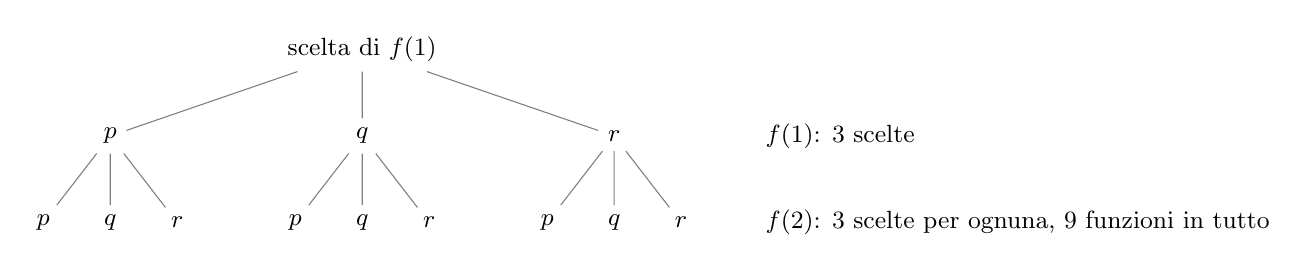
\begin{tikzpicture}[level distance=1.1cm, every node/.style={font=\small}, edge from parent/.style={draw=black!50},
                        level 1/.style={sibling distance=3.2cm}, level 2/.style={sibling distance=0.85cm}]
        \node {scelta di $f(1)$}
            child {node {$p$} child {node {$p$}} child {node {$q$}} child {node {$r$}}}
            child {node {$q$} child {node {$p$}} child {node {$q$}} child {node {$r$}}}
            child {node {$r$} child {node {$p$}} child {node {$q$}} child {node {$r$}}};
        \node[anchor=west, font=\small] at (5.0,-1.1) {$f(1)$: $3$ scelte};
        \node[anchor=west, font=\small] at (5.0,-2.2) {$f(2)$: $3$ scelte per ognuna, $9$ funzioni in tutto};
    \end{tikzpicture}
    \end{center}
    La biezione $\Psi$ della dimostrazione dice proprio questo: scegliere $f$ è come scegliere cosa fa sugli altri elementi
    ($f_{|a'}$) e, indipendentemente, dove manda $x$.
\end{spiegazione}

\begin{concetto}
\begin{Teorema}{Numero delle funzioni iniettive}{conta-iniettive}
    \begin{prerequisiti}
        \dip{Definizione}{def:fattoriale}
        \dip{Lemma}{lem:parti-finite}
        \dip{Lemma}{lem:somma-prodotto}
        \dip{Proposizione}{prop:ridotta}
        \dip{Teorema}{teo:comp-iniettive}
    \end{prerequisiti}
    Siano $|a| = m$ e $|b| = n$. Esistono funzioni iniettive da $a$ a $b$ se e solo se $m \leq n$, e in tal caso
    \[ |\mathrm{In}(a, b)| = \frac{n!}{(n - m)!} = n(n - 1) \cdots (n - m + 1). \]
\end{Teorema}
\begin{dimostrazione}
    \begin{caso}{$(\rightarrow)$ Se $f \in \mathrm{In}(a, b)$, allora $m \leq n$}
        La ridotta $a \to \mathrm{Im} f$ è biettiva, quindi $|\mathrm{Im} f| = m$; e $\mathrm{Im} f \subseteq b$, quindi $m \leq n$ (Lemma~\ref{lem:parti-finite}).
    \end{caso}
    \begin{caso}{$(\leftarrow)$ Se $m \leq n$, esistono funzioni iniettive}
        Siano $\alpha \colon a \to I_m$ e $\beta \colon b \to I_n$ biettive. Poiché $I_m \subseteq I_n$, l'immersione $\iota \colon I_m \to I_n$ è iniettiva,
        e $\beta^{-1} \circ \iota \circ \alpha \colon a \to b$ è iniettiva (composta di iniettive).
    \end{caso}
    \begin{caso}{Il conteggio, per induzione su $m \leq n$}
        Se $m = 0$, c'è solo la funzione vuota: $1 = n!/n!$. Se $m \geq 1$, sia $x \in a$ e $a' = a \setminus \{x\}$. Come nel teorema
        precedente, $f \mapsto (f_{|a'}, f(x))$ è una biezione tra $\mathrm{In}(a, b)$ e l'insieme delle coppie $(g, y)$ con $g \in \mathrm{In}(a', b)$ e
        $y \in b \setminus \mathrm{Im}\, g$ (perché $f$ resti iniettiva, $x$ deve andare in un elemento non ancora usato). Per ogni $g$ ci sono
        $|b \setminus \mathrm{Im}\, g| = n - (m - 1)$ scelte di $y$, quindi (Lemma~\ref{lem:somma-prodotto}, punto 3) e per ipotesi induttiva
        \[ |\mathrm{In}(a, b)| = \frac{n!}{(n - m + 1)!} \cdot (n - m + 1) = \frac{n!}{(n - m)!}. \]
    \end{caso}
\end{dimostrazione}
\end{concetto}

\begin{spiegazione}
    Ora le scelte \textbf{non} sono indipendenti: ogni elemento di $a$ deve andare in un elemento di $b$ non ancora usato. Il primo
    ha $n$ scelte, il secondo $n - 1$, \dots, l'$m$-esimo $n - m + 1$. Con $a = \{1, 2\}$ e $b = \{p, q, r\}$: $f(1)$ ha $3$ scelte, $f(2)$
    solo $2$, per un totale di $3 \cdot 2 = 6 = \frac{3!}{1!}$ funzioni iniettive. È il numero di modi di \textbf{ordinare} $m$ oggetti
    scelti tra $n$: ad esempio di assegnare oro e argento a $2$ dei $3$ concorrenti di una gara.
\end{spiegazione}

\begin{concetto}
\begin{Proposizione}{Esistenza di funzioni suriettive}{esistono-suriettive}
    \begin{prerequisiti}
        \dip{Teorema}{teo:suriettiva-sezione}
        \dip{Teorema}{teo:composte-caratteristiche}
        \dip{Teorema}{teo:conta-iniettive}
    \end{prerequisiti}
    Siano $|a| = m$ e $|b| = n$. Esistono funzioni suriettive da $a$ a $b$ se e solo se $a = b = \varnothing$ oppure $0 < n \leq m$.
\end{Proposizione}
\begin{dimostrazione}
    \begin{caso}{$(\rightarrow)$}
        Sia $f \colon a \to b$ suriettiva. Se $b = \varnothing$, anche $a = \varnothing$ (non ci sono funzioni da un insieme non vuoto al vuoto).
        Se $b \neq \varnothing$, $n > 0$; $f$ ha una sezione $g \colon b \to a$ (Teorema~\ref{teo:suriettiva-sezione}), e $f \circ g = \mathrm{id}_b$ è iniettiva,
        quindi $g$ è iniettiva (Teorema~\ref{teo:composte-caratteristiche}): per il Teorema~\ref{teo:conta-iniettive} $n \leq m$.
    \end{caso}
    \begin{caso}{$(\leftarrow)$}
        La funzione vuota da $\varnothing$ a $\varnothing$ è suriettiva. Se $0 < n \leq m$, la funzione $h \colon I_m \to I_n$ con $h(k) = k$ per $k \leq n$ e
        $h(k) = n$ per $k > n$ è suriettiva; componendo con biezioni $a \to I_m$ e $I_n \to b$ si ottiene una suriettiva da $a$ a $b$.
    \end{caso}
\end{dimostrazione}
\end{concetto}

\begin{spiegazione}
    Per «coprire» tutti gli $n$ elementi di $b$ servono almeno $n$ frecce che partono da elementi diversi, quindi almeno $n$
    elementi in $a$. Il caso $n = 0$ va trattato a parte: verso l'insieme vuoto parte solo la funzione vuota.
\end{spiegazione}

Quando $a$ e $b$ hanno lo stesso numero di elementi succede qualcosa di notevole.

\begin{concetto}
\begin{Teorema}{Iniettive, suriettive e biettive tra insiemi con lo stesso ordine}{stesso-ordine}
    \begin{prerequisiti}
        \dip{Teorema}{teo:ordine-finito}
        \dip{Proposizione}{prop:ridotta}
        \dip{Teorema}{teo:suriettiva-sezione}
        \dip{Teorema}{teo:composte-caratteristiche}
        \dip{Teorema}{teo:biettiva-inversa}
    \end{prerequisiti}
    Siano $a$ e $b$ finiti con $|a| = |b| = n$ e sia $f \colon a \to b$. Allora
    \[ f \text{ è iniettiva} \ \leftrightarrow\ f \text{ è biettiva} \ \leftrightarrow\ f \text{ è suriettiva}. \]
    Cioè $\mathrm{In}(a, b) = \mathrm{Bi}(a, b) = \mathrm{Su}(a, b)$.
\end{Teorema}
\begin{dimostrazione}
    Basta mostrare che ogni iniettiva e ogni suriettiva sono biettive.
    \begin{caso}{Iniettiva $\Rightarrow$ biettiva}
        La ridotta $a \to \mathrm{Im} f$ è biettiva, quindi $|\mathrm{Im} f| = n = |b|$. Se $\mathrm{Im} f$ fosse una parte propria di $b$, avrebbe ordine
        minore di $n$ (Teorema~\ref{teo:ordine-finito}, punto 3). Quindi $\mathrm{Im} f = b$: $f$ è suriettiva.
    \end{caso}
    \begin{caso}{Suriettiva $\Rightarrow$ biettiva}
        $f$ ha una sezione $g \colon b \to a$, con $f \circ g = \mathrm{id}_b$; $g$ è iniettiva (Teorema~\ref{teo:composte-caratteristiche}), quindi biettiva per il
        caso precedente (con i ruoli di $a$ e $b$ scambiati). Allora $f = f \circ g \circ g^{-1} = g^{-1}$ è biettiva.
    \end{caso}
\end{dimostrazione}
\end{concetto}

\begin{spiegazione}
    È il \textbf{principio dei cassetti}: se metto $n$ oggetti in $n$ cassetti senza mai metterne due nello stesso (iniettiva), li
    riempio tutti (suriettiva); e se li riempio tutti, non posso averne messi due nello stesso. Con gli insiemi infiniti è falso:
    \begin{itemize}
        \item $n \in \mbN \mapsto n + 1 \in \mbN$ è iniettiva ma non suriettiva ($0$ resta scoperto);
        \item $n \in \mbN \mapsto n - 1 \in \mbN$ per $n \geq 1$, con $0 \mapsto 0$, è suriettiva ma non iniettiva ($0$ e $1$ vanno entrambi in $0$).
    \end{itemize}
\end{spiegazione}

\begin{concetto}
\begin{Corollario}{Numero delle funzioni biettive}{conta-biettive}
    \begin{prerequisiti}
        \dip{Teorema}{teo:conta-iniettive}
        \dip{Teorema}{teo:stesso-ordine}
        \dip{Teorema}{teo:biettiva-inversa}
    \end{prerequisiti}
    Siano $|a| = m$ e $|b| = n$. Esistono funzioni biettive da $a$ a $b$ se e solo se $m = n$, e in tal caso $|\mathrm{Bi}(a, b)| = n!$.
    In particolare l'insieme $\mathrm{Bi}(a) := \mathrm{Bi}(a, a)$ delle biezioni di $a$ in sé (le \textbf{permutazioni} di $a$) ha $m!$ elementi.
\end{Corollario}
\begin{dimostrazione}
    Se $f \colon a \to b$ è biettiva, $f$ e $f^{-1}$ sono iniettive, quindi $m \leq n$ e $n \leq m$ (Teorema~\ref{teo:conta-iniettive}). Se $m = n$,
    per il Teorema~\ref{teo:stesso-ordine} $\mathrm{Bi}(a, b) = \mathrm{In}(a, b)$, che ha $\frac{n!}{(n - n)!} = \frac{n!}{0!} = n!$ elementi.
\end{dimostrazione}
\end{concetto}

\begin{spiegazione}
    Le permutazioni di $\{1, 2, 3\}$ sono $3! = 6$: il primo posto si sceglie in $3$ modi, il secondo in $2$, il terzo in $1$. Eccole,
    scritte come la sequenza $f(1)f(2)f(3)$: \quad $123$, \ $132$, \ $213$, \ $231$, \ $312$, \ $321$.
\end{spiegazione}

% ──────────────────────────────────────────────────────────────
\section{Insiemi infiniti a confronto}\label{sec:confronto-infiniti}

Anche tra insiemi infiniti si possono confrontare le «grandezze» con le biezioni. Qui diamo solo qualche cenno.

\begin{concetto}
\begin{Proposizione}{$\mbN$ e $\mbZ$ sono equipotenti}{n-z}
    \begin{prerequisiti}
        \dip{Definizione}{def:equipotenti}
        \dip{Teorema}{teo:biettiva-inversa}
    \end{prerequisiti}
    La funzione $f \colon \mbN \to \mbZ$ definita da $f(n) = -\frac{n}{2}$ se $n$ è pari e $f(n) = \frac{n + 1}{2}$ se $n$ è dispari è biettiva.
\end{Proposizione}
\begin{dimostrazione}
    Sia $g \colon \mbZ \to \mbN$ con $g(z) = -2z$ se $z \leq 0$ e $g(z) = 2z - 1$ se $z > 0$. Se $n$ è pari, $f(n) = -\frac{n}{2} \leq 0$ e
    $g(f(n)) = n$; se $n$ è dispari, $f(n) = \frac{n + 1}{2} > 0$ e $g(f(n)) = n$. Se $z \leq 0$, $g(z) = -2z$ è pari e $f(g(z)) = z$; se $z > 0$,
    $g(z) = 2z - 1$ è dispari e $f(g(z)) = z$. Quindi $g$ è l'inversa di $f$, e $f$ è biettiva (Teorema~\ref{teo:biettiva-inversa}).
\end{dimostrazione}
\end{concetto}

\begin{spiegazione}
    Sembra che $\mbZ$ abbia «il doppio» degli elementi di $\mbN$, eppure si possono elencare tutti gli interi in una sola fila,
    \textbf{a zig-zag}: $0, 1, -1, 2, -2, 3, -3, \dots$ È quello che fa $f$:
    \begin{center}
    \renewcommand{\arraystretch}{1.2}
    \begin{tabular}{c|ccccccccc}
        $n$ & $0$ & $1$ & $2$ & $3$ & $4$ & $5$ & $6$ & $7$ & $\cdots$ \\ \hline
        $f(n)$ & $0$ & $1$ & $-1$ & $2$ & $-2$ & $3$ & $-3$ & $4$ & $\cdots$ \\
    \end{tabular}

    \medskip
    \begin{tikzpicture}[x=1.0cm]
        \foreach \z in {-3,...,3} \node[circle, draw=black!40, fill=primary!7, inner sep=0pt, minimum size=6.5mm, font=\small] (z\z) at (\z,0) {$\z$};
        \foreach \a/\b in {0/1, 1/-1, -1/2, 2/-2, -2/3, 3/-3}
            \draw[-{Stealth}, orange!80!black, line width=0.7pt] (z\a) to[bend left=50] (z\b);
        \node[font=\small, anchor=west] at (3.8,0) {la spirale tocca ogni intero una volta sola};
    \end{tikzpicture}
    \end{center}
\end{spiegazione}

\begin{concetto}
\begin{Teorema}{Teorema di Cantor}{cantor}
    \begin{prerequisiti}
        \dip{Definizione}{def:suriettiva}
        \dip{Assioma}{ass:separazione}
    \end{prerequisiti}
    Per nessun insieme $a$ esiste una funzione suriettiva da $a$ a $\mcP(a)$. In particolare $\mbN$ e $\mcP(\mbN)$ non sono equipotenti.
\end{Teorema}
\begin{dimostrazione}
    \facoltativa
    Per assurdo sia $f \colon a \to \mcP(a)$ suriettiva e sia $d = \{x \in a \mid x \notin f(x)\}$. Poiché $d \in \mcP(a)$, esiste $y \in a$ con
    $f(y) = d$. Allora $y \in d \leftrightarrow y \notin f(y) \leftrightarrow y \notin d$: assurdo.
\end{dimostrazione}
\end{concetto}

\begin{spiegazione}
    Ogni elemento $x$ «propone» una parte $f(x)$; la parte $d$ è costruita per essere \textbf{diversa da tutte le proposte}: per
    ogni $x$, $d$ e $f(x)$ non sono d'accordo proprio su $x$. Quindi nessuno propone $d$. È lo stesso trucco del paradosso di
    Russell, e dice che esistono infiniti «più grandi» di altri: $\mcP(\mbN)$ non si può elencare in una fila come $\mbN$.
\end{spiegazione}

% ──────────────────────────────────────────────────────────────
\section{Funzioni caratteristiche e insieme delle parti}\label{sec:caratteristiche}

\dfn[funzione-caratteristica]{Funzione caratteristica}{
    Sia $s$ un insieme e $t \subseteq s$. La funzione
    \[ \chi_{t, s} \colon x \in s \mapsto \begin{cases} 1 & \text{se } x \in t \\ 0 & \text{se } x \notin t \end{cases} \in \{0, 1\} \]
    si chiama \textbf{funzione caratteristica} di $t$ in $s$.
}

\begin{concetto}
\begin{Teorema}{Parti e funzioni caratteristiche}{parti-caratteristiche}
    \begin{prerequisiti}
        \dip{Definizione}{def:funzione-caratteristica}
        \dip{Definizione}{def:biettiva}
        \dip{Corollario}{cor:terna}
    \end{prerequisiti}
    Sia $s$ un insieme. La funzione $\varphi \colon t \in \mcP(s) \mapsto \chi_{t, s} \in \mathrm{Map}(s, \{0, 1\})$ è biettiva.
\end{Teorema}
\begin{dimostrazione}
    \begin{caso}{Suriettiva}
        Sia $f \in \mathrm{Map}(s, \{0, 1\})$ e sia $t = \{x \in s \mid f(x) = 1\}$. Per $x \in t$, $\chi_{t, s}(x) = 1 = f(x)$; per $x \in s \setminus t$,
        $\chi_{t, s}(x) = 0 = f(x)$. Le due funzioni hanno lo stesso grafico, quindi $\varphi(t) = \chi_{t, s} = f$.
    \end{caso}
    \begin{caso}{Iniettiva}
        Siano $t \neq u$ parti di $s$: senza perdere di generalità esiste $x \in t \setminus u$. Allora $\chi_{t, s}(x) = 1 \neq 0 = \chi_{u, s}(x)$, quindi
        $\chi_{t, s} \neq \chi_{u, s}$.
    \end{caso}
\end{dimostrazione}
\end{concetto}

\begin{spiegazione}
    Una parte di $s$ è una lista di risposte «sì/no» alla domanda «$x$ sta in $t$?», una per ogni elemento di $s$. Se gli elementi
    di $s$ sono messi in fila, è una \textbf{stringa di bit}. Per $s = \{a, b, c\}$:
    \begin{center}
    \renewcommand{\arraystretch}{1.2}
    \begin{tabular}{c|cccccccc}
        $t$ & $\varnothing$ & $\{c\}$ & $\{b\}$ & $\{b, c\}$ & $\{a\}$ & $\{a, c\}$ & $\{a, b\}$ & $\{a, b, c\}$ \\ \hline
        $\chi_{t, s}(a)\,\chi_{t, s}(b)\,\chi_{t, s}(c)$ & $000$ & $001$ & $010$ & $011$ & $100$ & $101$ & $110$ & $111$ \\
    \end{tabular}
    \end{center}
    Le parti e le stringhe si corrispondono una a una: è l'idea con cui un computer memorizza un sottoinsieme.
\end{spiegazione}

\begin{concetto}
\begin{Corollario}{Le parti di un insieme finito}{cardinalita-parti}
    \begin{prerequisiti}
        \dip{Teorema}{teo:parti-caratteristiche}
        \dip{Teorema}{teo:conta-map}
    \end{prerequisiti}
    Se $|s| = n$, allora $|\mcP(s)| = 2^n$.
\end{Corollario}
\begin{dimostrazione}
    Per il Teorema~\ref{teo:parti-caratteristiche} $\mcP(s)$ è equipotente a $\mathrm{Map}(s, \{0, 1\})$, che ha $2^n$ elementi per il
    Teorema~\ref{teo:conta-map}.
\end{dimostrazione}
\end{concetto}

\begin{spiegazione}
    Si può vedere anche per induzione: le parti di $s \cup \{x\}$ (con $x \notin s$) sono quelle che \textbf{non} contengono $x$, cioè le
    parti di $s$, e quelle che lo contengono, ottenute aggiungendo $x$ a una parte di $s$. Ogni elemento in più \textbf{raddoppia} il
    numero delle parti: $2^n + 2^n = 2^{n + 1}$.
    \begin{center}
    \begin{tikzpicture}[every node/.style={font=\small}]
        \node[hv] at (0,0) {$\varnothing$}; \node[hv] at (1.0,0) {$\{a\}$}; \node[hv] at (2.0,0) {$\{b\}$}; \node[hv] at (3.2,0) {$\{a, b\}$};
        \node[hv evid] at (0,-0.9) {$\{c\}$}; \node[hv evid] at (1.15,-0.9) {$\{a, c\}$}; \node[hv evid] at (2.4,-0.9) {$\{b, c\}$};
        \node[hv evid] at (3.75,-0.9) {$\{a, b, c\}$};
        \node[anchor=west] at (4.8,0) {parti di $\{a, b\}$: $4$};
        \node[anchor=west] at (4.8,-0.9) {le stesse con $c$ aggiunto: altre $4$};
    \end{tikzpicture}
    \end{center}
\end{spiegazione}

% ──────────────────────────────────────────────────────────────
\section{Monoidi e anelli finiti}\label{sec:monoidi-finiti}

Nel Capitolo~\ref{cap:gruppi} abbiamo visto che in un monoide ogni elemento invertibile è cancellabile, ma che il viceversa è
falso in generale (in $(\mbZ, \cdot, 1)$ il $2$ è cancellabile ma non invertibile). Negli insiemi finiti il
Teorema~\ref{teo:stesso-ordine} ribalta la situazione.

\begin{concetto}
\begin{Teorema}{Monoide finito: invertibile se e solo se cancellabile}{monoide-finito}
    \begin{prerequisiti}
        \dip{Teorema}{teo:invertibile-cancellabile}
        \dip{Proposizione}{prop:traslazioni}
        \dip{Teorema}{teo:stesso-ordine}
        \dip{Teorema}{teo:unicita-inverso}
    \end{prerequisiti}
    Sia $(m, *, 1_m)$ un monoide finito. Allora $a \in m$ è invertibile se e solo se $a$ è cancellabile.
\end{Teorema}
\begin{dimostrazione}
    \begin{caso}{$(\rightarrow)$ Se $a$ è invertibile, allora è cancellabile}
        È il Teorema~\ref{teo:invertibile-cancellabile}.
    \end{caso}
    \begin{caso}{$(\leftarrow)$ Se $a$ è cancellabile, allora è invertibile}
        Le traslazioni $\sigma_a$ e $\delta_a$ sono iniettive (Proposizione~\ref{prop:traslazioni}). Sono funzioni dall'insieme finito $m$ in sé,
        quindi sono anche suriettive (Teorema~\ref{teo:stesso-ordine}). Allora esistono $b, c \in m$ con
        \[ \sigma_a(b) = a * b = 1_m \qquad\qquad \delta_a(c) = c * a = 1_m: \]
        $a$ ha un inverso destro e uno sinistro, quindi è invertibile (e $b = c$ per il Teorema~\ref{teo:unicita-inverso}).
    \end{caso}
\end{dimostrazione}
\end{concetto}

\begin{spiegazione}
    Sulla tavola di Cayley: $a$ cancellabile a sinistra vuol dire che nella riga di $a$ non ci sono ripetizioni
    (Proposizione~\ref{prop:lettura-cayley}). Se la tavola è finita, una riga di $n$ caselle senza ripetizioni contiene
    \textbf{tutti} gli $n$ elementi, quindi anche $1_m$: e la colonna in cui compare $1_m$ è l'inverso destro di $a$. In $(\mbZ, \cdot)$ la
    riga del $2$ ($\dots, -2, 0, 2, 4, \dots$) non ha ripetizioni ma, essendo infinita, può «saltare» l'$1$.
\end{spiegazione}

\begin{concetto}
\begin{Teorema}{Anelli integri finiti}{integri-finiti}
    \begin{prerequisiti}
        \dip{Teorema}{teo:monoide-finito}
        \dip{Teorema}{teo:divisori-cancellabili}
        \dip{Definizione}{def:corpo-campo}
        \dip{Definizione}{def:lap}
        \dip{Lemma}{lem:regole-anello}
    \end{prerequisiti}
    Sia $(a, +, \cdot)$ un anello unitario finito, integro, con almeno due elementi. Allora $a$ è un corpo.
    In particolare, ogni dominio di integrità finito è un campo.
\end{Teorema}
\begin{dimostrazione}
    \begin{caso}{$(a \setminus \{0_a\}, \cdot, 1_a)$ è un monoide}
        $1_a \neq 0_a$ (Lemma~\ref{lem:regole-anello}, punto 4), quindi $1_a \in a \setminus \{0_a\}$. Per la LAP, se $x, y \neq 0_a$ allora $xy \neq 0_a$:
        $a \setminus \{0_a\}$ è una parte chiusa di $(a, \cdot)$.
    \end{caso}
    \begin{caso}{Ogni suo elemento è invertibile}
        Sia $x \neq 0_a$. Per la LAP $x$ non è divisore dello zero, quindi è cancellabile (Teorema~\ref{teo:divisori-cancellabili}), anche nel
        monoide finito $a \setminus \{0_a\}$. Per il Teorema~\ref{teo:monoide-finito} $x$ è invertibile. Quindi $(a \setminus \{0_a\}, \cdot)$ è un gruppo:
        $a$ è un corpo. Se $a$ è anche commutativo (dominio di integrità), è un campo.
    \end{caso}
\end{dimostrazione}
\end{concetto}

\begin{spiegazione}
    In un anello integro moltiplicare per $x \neq 0$ non «schiaccia» mai due elementi diversi nello stesso risultato
    ($xy = xz \Rightarrow y = z$). Se gli elementi sono finiti, moltiplicare per $x$ è quindi una permutazione degli elementi non nulli,
    e prima o poi si ottiene $1$: lì c'è l'inverso di $x$. Vedremo nel Capitolo~\ref{cap:congruenze} gli esempi più importanti:
    gli anelli $\mbZ_p$ con $p$ primo.
\end{spiegazione}
